% !TeX root = RJwrapper.tex
\title{\pkg{sejmRP}: An Information About Polish Diet - DRAFT}
\author{by Piotr Smuda, Przemysław Biecek}

\maketitle

%An abstract of less than 150 words.
\abstract{
The \pkg{sejmRP} package provides a set of functions, that can be used to scrap data from Polish Diet's webpage \url{http://www.sejm.gov.pl/} about deputies, votings and deputies' statements from seventh to eighth term of office. All data is storaged in PostgreSQL database, which enables easier access to it and possibility of its analysis.}

\section{Introduction}

Nowadays, in times of open government...

\section{User manual}

\subsection{Functions}

\begin{table}[h]
\centering
\begin{tabular}{|l||c|c|c|} \hline
subject & database & deputies & votings \\ \hline
scraping functions & create\_database & deputies\_create\_table & votings\_create\_table \\
 & remove\_database & deputies\_update\_table & votings\_update\_table \\
 & & deputies\_add\_new & votings\_get\_date \\
 & & deputies\_get\_data & votings\_get\_meetings\_links \\
 & & deputies\_get\_ids & votings\_get\_meetings\_table \\
 & & & votings\_get\_votings\_links \\
 & & & votings\_get\_votings\_table \\ \hline
access functions & & get\_deputies\_table & get\_votings\_table \\ \hline
\end{tabular}
\\
\begin{tabular}{|c|c|} \hline
votes & statements \\ \hline
votes\_create\_table & statements\_create\_table \\
votes\_update\_table & statements\_update\_table\\
votes\_get\_clubs\_links & statements\_get\_statement \\
votes\_get\_results & statements\_get\_statements\_data \\
votes\_match\_deputies\_ids & statements\_get\_statements\_table \\ \hline
get\_votes\_table & get\_statements\_table \\
get\_filtered\_votes & \\ \hline
\end{tabular}
\caption{List of functions for each table from database.}
\label{tab:getdatatable}
\end{table}

\subsection{Structure of database}

\begin{figure}[htbp]
  \centering
  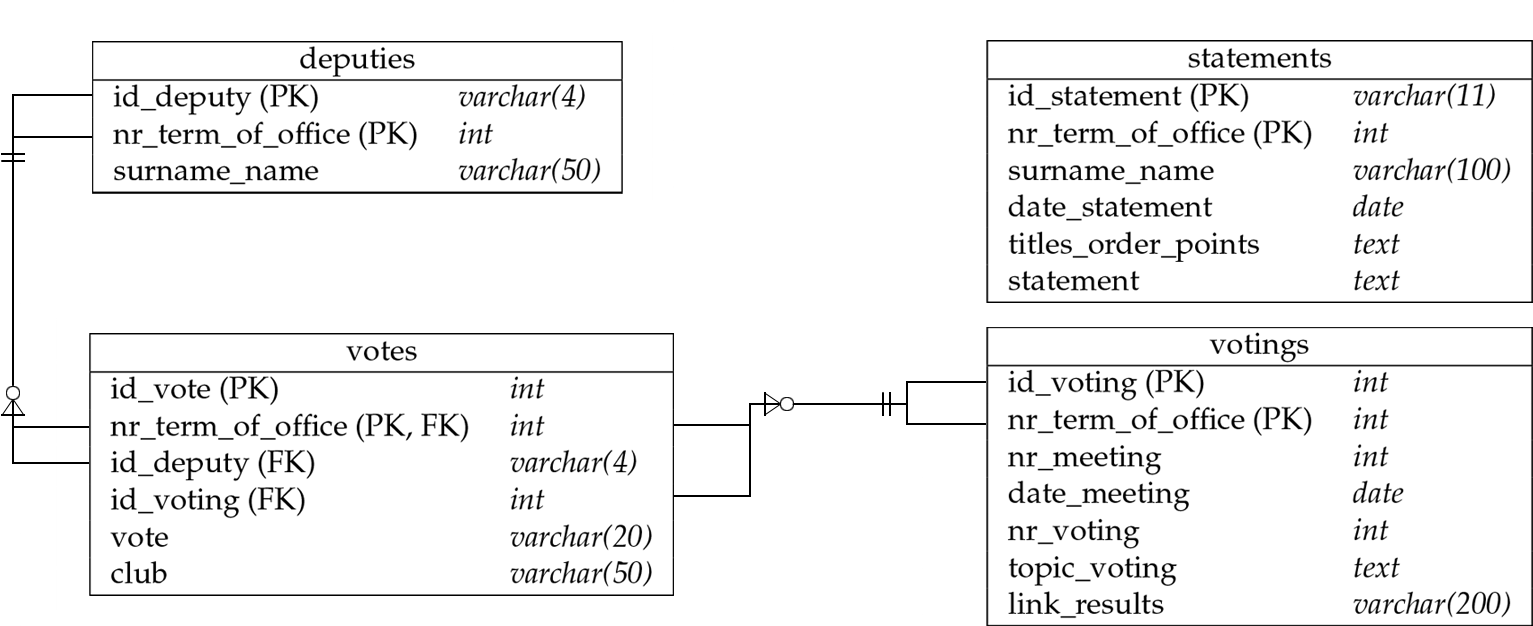
\includegraphics{erd}
  \caption{ERD of database.}
  \label{figure:erd}
\end{figure}


\section{Use-cases}


\section{Summary}



\bibliography{smuda-biecek}

\address{Piotr Smuda\\
  Faculty of Mathematics and Information Science\\
  Warsaw University of Technology\\
  Koszykowa 75, 00-662 Warsaw\\
  Poland\\}
\email{smudap@student.mini.pw.edu.pl}

\address{Przemysław Biecek\\
  Faculty of Mathematics and Information Science\\
  Warsaw University of Technology\\
  Koszykowa 75, 00-662 Warsaw\\
  Poland\\}
\email{przemyslaw.biecek@mini.pw.edu.pl}
